\chapter{Технологический раздел}

\section{Выбор средств программной реализации}

В качестве языка программирования был выбран язык \textit{Python3}. Это скриптовый язык с динамической типизацией, что позволяет ускорить процесс разработки, а программу можно запускать на любом компьютере, где есть интерпретатор \textit{Python3}.

\section{Сборка инструмента}

Для того, чтобы запустить разработанный инструмент, необходимо:
\begin{enumerate}
\item установить интерпретатор \textit{Python3},

\item установить пакетный менеджер \textit{pip} для \textit{Python3},

\item установить модуль \textit{sqlparse}, для парсинга SQL запросов: \\\textit{pip install --upgrade sqlparse}

\item скачать скрипты по адресу:\\ \textit{https://github.com/iproha94/mysql-indexes/tree/master/src}
\end{enumerate}

\section{Руководство пользователя}

\paragraph{Процесс использования ПО АБД}

\begin{enumerate}
\item подготовить входной файл с SQL запросами, для которых необходимо построить индексы. Каждый SQL запрос должен быть на одной строке, и заканчиваться переводом строки. Каждый знак сравнения должен быть обрамлен пробелами. 

\item запустить скрипт \textit{index_advisor} с указанием пути входного файла (например \ref{example-input-file})\\ \textit{python3 index_advisor.py example.sql}

\item результаты работы программы будут в сгенерированном выходном файле (например \ref{example-output-file}). В нем для каждого успешно считанного SQL запроса будут сгенерированы SQL строки с созданием рекомендуемого индекса.
\end{enumerate}


\begin{lstlisting}[language=sql, caption={Пример входного файла},label=example-input-file]
select * FROM t1 LEFT JOIN t2 ON t1.a = t2.a WHERE t1.b > 1 AND t2.c = 5;
select * FROM t1 LEFT JOIN t2 ON t1.a = t2.a WHERE t1.b = 5000 AND t1.c > 3 ORDER BY t2.c , t2.d;
select * FROM t1 LEFT JOIN t2 ON t1.a = t2.a WHERE t2.b = 5000 AND t2.c > 3 ORDER BY t2.c, t2.d;
select * FROM t1 LEFT JOIN t2 ON t2.a = t1.a ORDER BY t2.b"
select * FROM t1 INNER JOIN t2 ON t1.a = t2.a WHERE t1.b = 5 ORDER BY t1.c;
select * from t where a = 5 and b > 1;
select * from t where a = 5 and c = 5;
select * from t where a = 5 and c > 3 and b = 5000;
select * from t where a = 5;
select * from t where b = 5 and a = 5 and c > 3 order by c, d;
\end{lstlisting}

\begin{lstlisting}[language=sql, caption={Пример выходного файла},label=example-output-file]
select * FROM t1 LEFT JOIN t2 ON t1.a = t2.a WHERE t1.b > 1 AND t2.c = 5;
CREATE INDEX index_t1_ab t1(a, b); 
CREATE INDEX index_t2_c t2(c);

CREATE INDEX index_t1_b t1(b); 
CREATE INDEX index_t2_ac t2(a, c);

select * FROM t1 LEFT JOIN t2 ON t1.a = t2.a WHERE t1.b = 5000 AND t1.c > 3 ORDER BY t2.c , t2.d;
CREATE INDEX index_t1_bc t1(b, c);
CREATE INDEX index_t2_a t2(a);

select * FROM t1 LEFT JOIN t2 ON t1.a = t2.a WHERE t2.b = 5000 AND t2.c > 3 ORDER BY t2.c, t2.d;
CREATE INDEX index_t1_a t1(a);
CREATE INDEX index_t2_bcd t2(b, c, d);

select * FROM t1 LEFT JOIN t2 ON t2.a = t1.a ORDER BY t2.b;
CREATE INDEX index_t2_a t2(a);

select * FROM t1 INNER JOIN t2 ON t1.a = t2.a WHERE t1.b = 5 ORDER BY t1.c;
CREATE INDEX index_t1_bc t1(b, c); 
CREATE INDEX index_t2_a t2(a);

select * from t where a = 5 and b > 1;
CREATE INDEX index_t_ab t(a, b);

select * from t where a = 5 and c = 5;
CREATE INDEX index_t_ac t(a, c);

select * from t where a = 5 and c > 3 and b = 5000;
CREATE INDEX index_t_abc t(a, b, c)

select * from t where a = 5;
CREATE INDEX index_t_a t(a);

select * from t where b = 5 and a = 5 and c > 3 order by c, d;
CREATE INDEX index_t_bacd t(b, a, c, d);
\end{lstlisting}


\paragraph{Процесс использования ПО другими приложениями}

\begin{enumerate}
\item запустить скрипт \textit{simple_query} или \textit{join_query}, первым аргументом передав строку с простым или сложным SQL запросом соответственно. Например \ref{img:example_simple_query}, \ref{img:example_join_query} :\\
\textit{python3 simple_query.py "select * from t where a = 5 and b > 1"} \\
\textit{python3 join_query.py "select * FROM t1 INNER JOIN t2 ON t1.a = t2.a WHERE t1.b = 5 ORDER BY t1.c"}

\item в результате работы в выводе будет строка с SQL запросом для создания индекса. При ошибке в работе программы код возврата будет отличным от нуля.
\end{enumerate}

\begin{figure}[h]
  \centering
  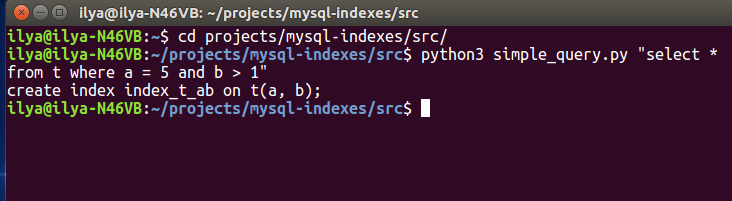
\includegraphics[scale=0.5]{example-simple-query.png}
  \caption{Пример запуска скрипта simple_query.py}
  \label{img:example_simple_query}
\end{figure}

\begin{figure}[h]
  \centering
  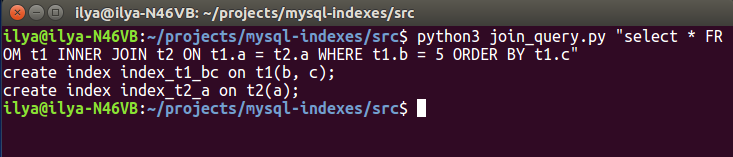
\includegraphics[scale=0.5]{example-join-query.png}
  \caption{Пример запуска скрипта join_query.py}
  \label{img:example_join_query}
\end{figure}
